\subsection*{a}
\begin{figure}[h!]
	\centering
	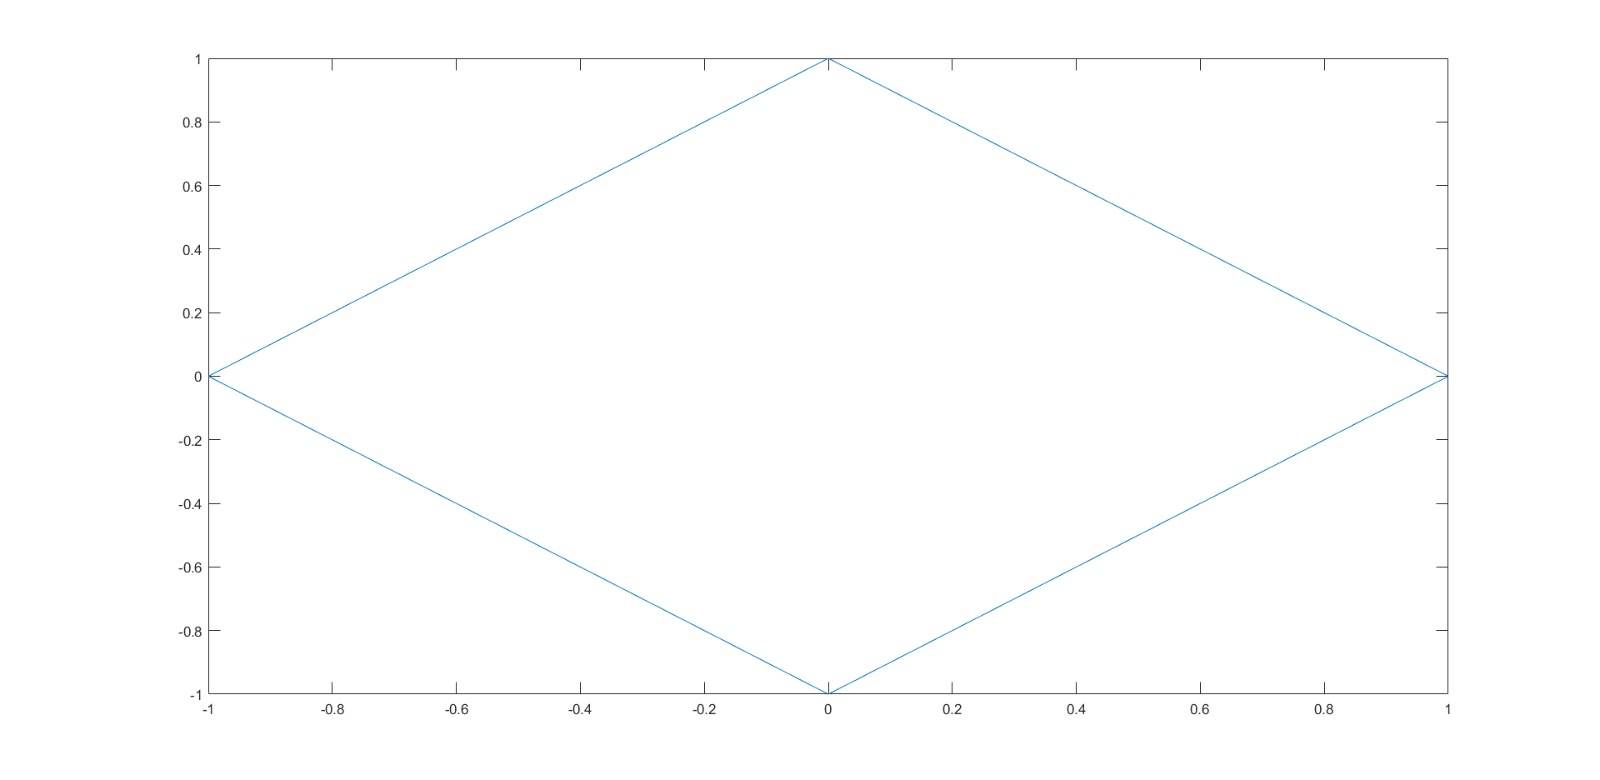
\includegraphics[width=\linewidth]{2dL1unitball.jpeg}
	\caption{$B^2_1$ unit ball}
	\label{fig:b21ub}
\end{figure}
$B^3_1$ can be represented the intersection of half-spaces $\pm x \pm y \pm z \leq 1$. Thus the unit ball is limited by 8 planes  $\pm x \pm y \pm z \leq 1$. The image of a $B^3_1$ unit ball is on \ref{fig:b31ub}.
\begin{figure}[h!]1
	\centering
	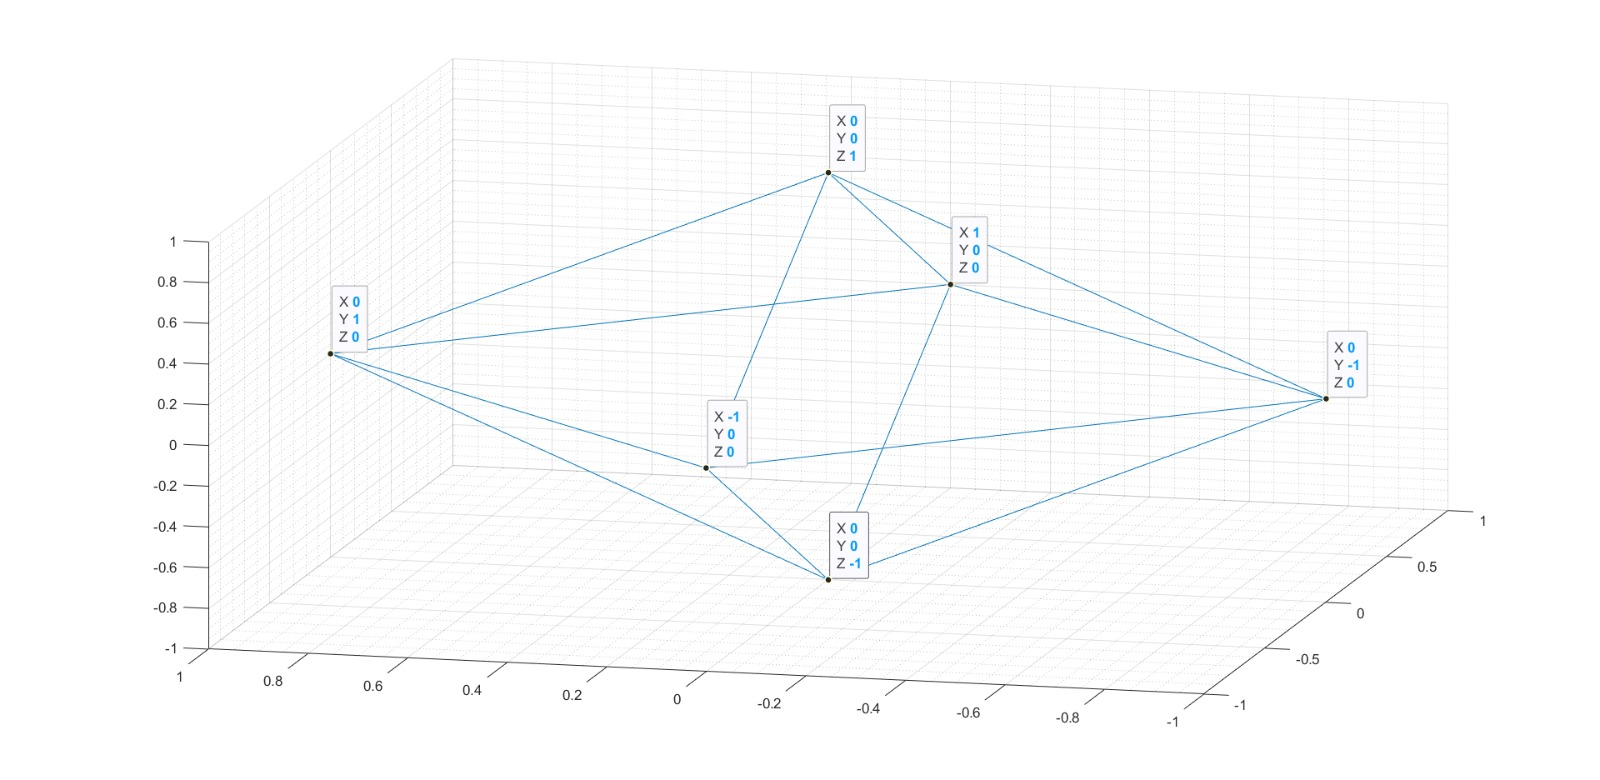
\includegraphics[width=\linewidth]{3dL1unitball.jpeg}
	\caption{$B^3_1$ unit ball}
	\label{fig:b31ub}
\end{figure}

\subsection*{b}
$vol(B^2_1) = \text{sum of areas of 4 rectangular triangles with unit side size} = 4 \cdot \dfrac{1}{2} \cdot 1 \cdot 1$
$vol(B^3_1) = \text{sum of 8 volumes of tetrahedral with tip in the origin} = 8 \cdot \dfrac{1}{3} \cdot 1 \cdot \dfrac{1}{2} = \dfrac{4}{3}$
\subsection*{d}
Suppose each $B^l_1$ unit sphere limited by $2k$ prisms with thickness $t = \dfrac{1}{k}$ and width $w_i = (1 - i*t) \forall i \in \{1, .. , k\}: \text{index of a prism from the equator}$.\\
Thus the volume of i-th l-dimensional prism is $t \cdot (1 - i\cdot t)^{l-1} \cdot vol(B^{l-1}_1)$, and therefore
$vol(B^l_1) \leq 2\cdot \sum_{i=1}^{k}(t \cdot (1 - i\cdot t)^{l-1} \cdot vol(B^{l-1}_1)) = 
	2\cdot \dfrac{1}{k} \cdot \sum_{i = 1}^{k}
	(1 - i\cdot \dfrac{1}{k})^{l-1} \cdot 
	vol(B^{l-1}_1)
$. To prove, that $\lim_{l \to \infty} vol(B^l) = 0$ we need to prove, that for some $\exists k\in N_{>0}, c \in (0,1), n : \forall l > n \implies f_k(l) \leq c$ where $f_k(l) = 2\cdot \dfrac{1}{k} \cdot \sum_{i=1}^{k} (1 - i\cdot \dfrac{1}{k})^{l-1}$.\\ 
Let's take $k = 2$ and $c = 0.5$. Then $f_2(l) = \sum_{i = 1}^{2} (1 - \dfrac{i}{2})^{l-1} \leq 2\cdot 0.5^{l-1}$. Taking $l > 3 \implies 2\cdot 0.5^{l-1} < 0.5$, which proofs, that  $\forall l > 3: f_2(l) \leq c $ and consequently $\lim_{l \to \infty} vol(B^l) = 0$.